\def\baselinestretch{1}
\chapter{Observations} \label{Observations chapter}
\ifpdf
    \graphicspath{{Conclusions/ConclusionsFigs/PNG/}{Conclusions/ConclusionsFigs/PDF/}{Conclusions/ConclusionsFigs/}}
\else
    \graphicspath{{Conclusions/ConclusionsFigs/EPS/}{Conclusions/ConclusionsFigs/}}
\fi

\def\baselinestretch{1.66}

\section{Part 1 -- W-Net}\label{sec:ob_wnet}

We experimented with two different model architectures; W-Net Combined and W-Net 3-layer. We discuss the observations relating to these below, against W-Net\footnote{W-Net comparison model taken from \underline{\href{https://github.com/rmsouza01/Hybrid-CS-Model-MRI}{rmsouza01's GitHub page}}}. The input was corrupted in the k-space domain for training and testing using a random 80\% undersampling mask (example in fig \ref{k-space mask}) to retain only 20\% of the k-space data.


\begin{figure}[!htbp]
  \begin{center}
    \leavevmode
    \ifpdf
      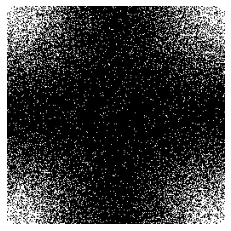
\includegraphics[height=1.5in]{Chapter4/images/k-space-mask.png}
    \else
      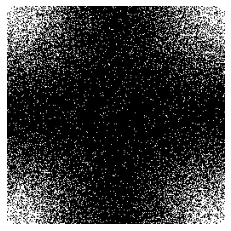
\includegraphics[bb = 92 86 545 742, height=3in]{Chapter4/images/k-space-mask.png}
    \fi
    \caption{80 \% undersampling mask for k-space}
    \label{k-space mask}
  \end{center}
\end{figure}



\vspace*{0.3cm}
\begin{table}[h]
\begin{center}
\begin{tabular}{ p{4cm} m{3cm} m{3cm} m{3cm} }
 \hline
 \multicolumn{4}{c}{Comparison table -- W-Net models} \\
 \hline
 & PSNR & SSIM & Parameters \\
 \hline
 \hline
 \textbf{W-Net}    & $33.24 \pm 2.92$ & 0.8829 & 4M\\
 \hline
 \textbf{W-Net Combined}& $31.22 \pm 3.28 $& 0.7832 & 2+2+4 M\\
 \textbf{W-Net 3-layer}& $32.21 \pm 0.53$  & 0.8385 & 4M\\
 \hline
\end{tabular}
\end{center}
\caption{Comparison between W-Net models}
\label{W-Net table}
\end{table}

\subsection{W-Net Combined}


\vspace*{0.5cm}
\begin{figure}[!htbp]
  \begin{center}
    \leavevmode
    \ifpdf
      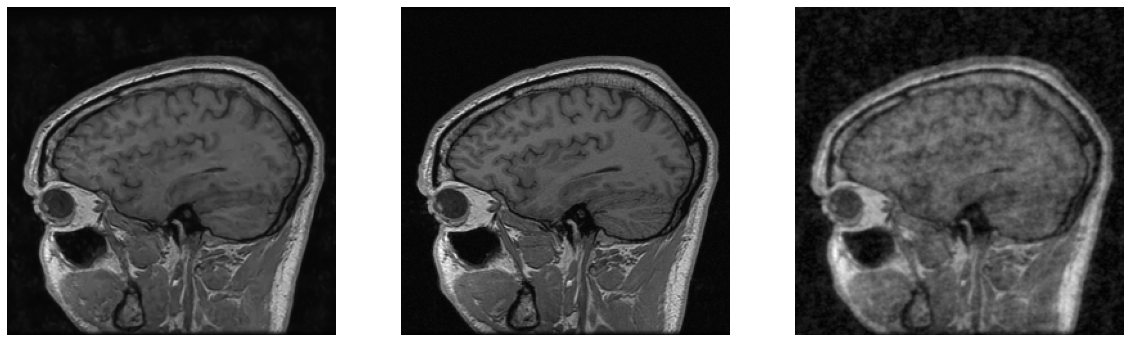
\includegraphics[height=1.5in]{Chapter4/images/res1.png}
    \else
      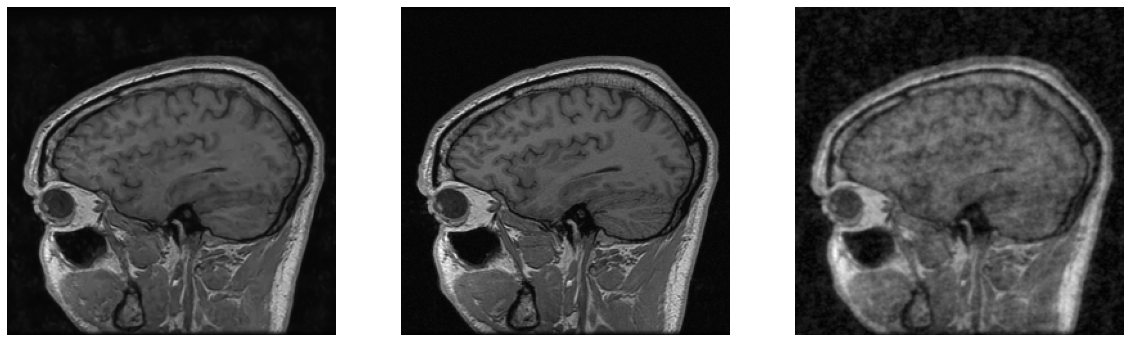
\includegraphics[bb = 92 86 545 742, height=3in]{Chapter4/images/res1.png}
    \fi
    % \caption{Result 1 }
    % \label{Result 1 W-Net Combined}
  \end{center}

  \begin{center}
    \leavevmode
    \ifpdf
      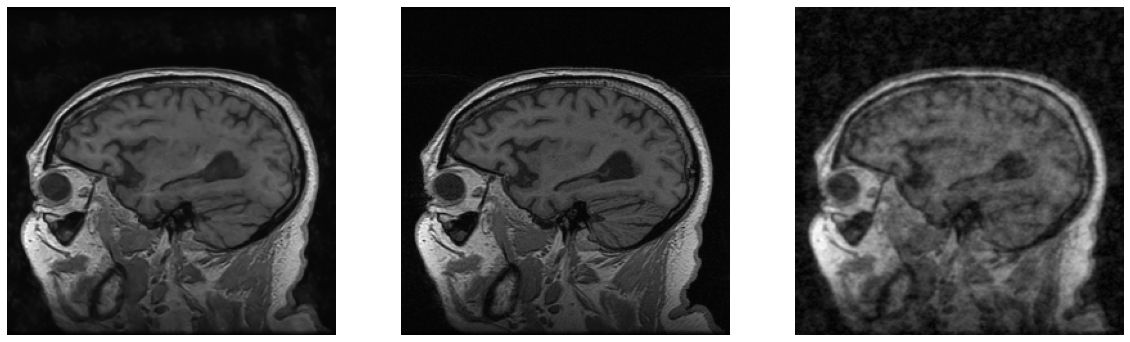
\includegraphics[height=1.5in]{Chapter4/images/res2.png}
    \else
      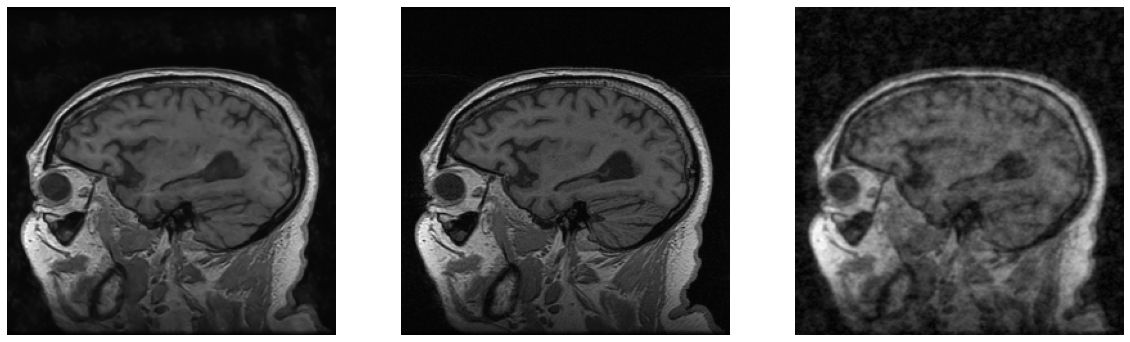
\includegraphics[bb = 92 86 545 742, height=3in]{Chapter4/images/res2.png}
    \fi
    \caption{W-Net Combined results -- Predicted (Left), Original (Middle), Undersampled (Right)}
    \label{Result W-Net Combined}
  \end{center}
\end{figure}

We trained Part 1 (k-space domain) and Part 2 (image domain) of the models separately for 20 epochs each on the k-space data for 25 MRIs, with 10 for validation, and finally trained the whole combined model by joining the two previously trained parts for 15 epochs. Each MRI contained around 170 image slices. The training was done on a Tesla T4 GPU.\\

We don't have comparisons to other super-resolution algorithms such as EDSR or Bicubic interpolation because the image was corrupted in the k-space domain and retains the same pixel dimensions as the original. This is MR reconstruction rather than super-resolution.\\

We can see from figure \ref{Result W-Net Combined} that a lot of the fine details are visible in the prediction and is very true to the original. The PSNR is very close (table \ref{W-Net table}) to the original W-Net, all while using significantly lesser computational time because of the split training technique. We believe that this model is an improvement over the original W-Net as it gives comparable results while reducing the training time and hardware requirements.


\subsection{W-Net 3-layer}

\vspace*{0.5cm}
\begin{figure}[!htbp]
  \begin{center}
    \leavevmode
    \ifpdf
      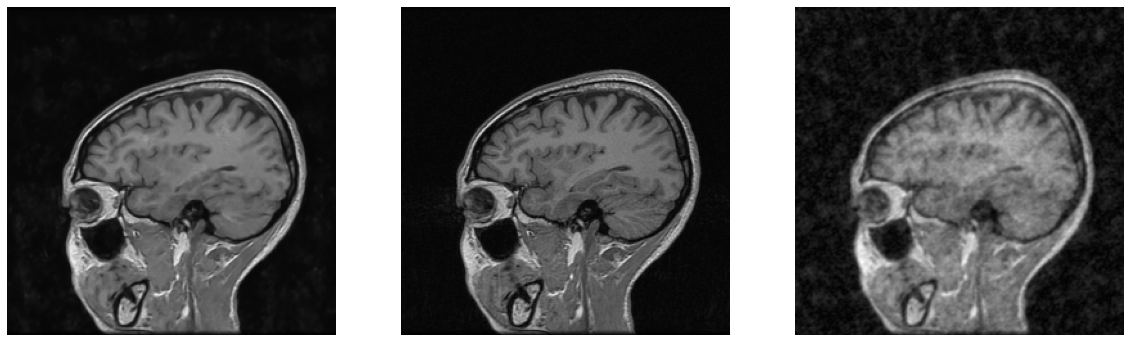
\includegraphics[height=1.5in]{Chapter4/images/res3.png}
    \else
      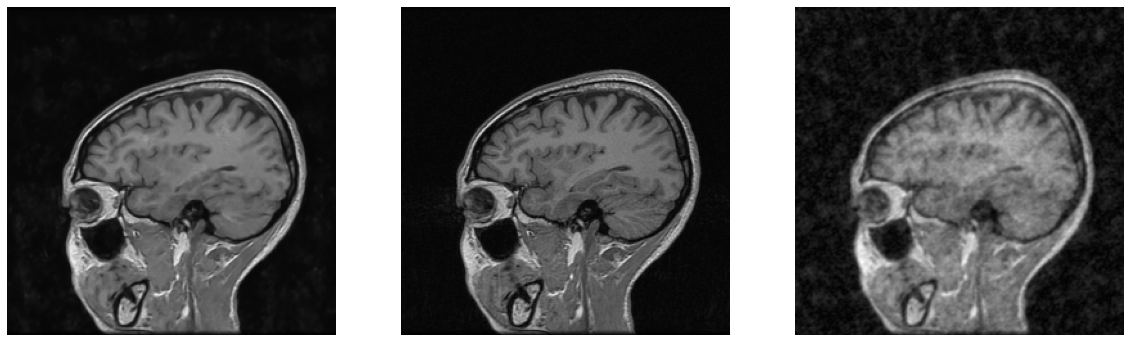
\includegraphics[bb = 92 86 545 742, height=3in]{Chapter4/images/res3.png}
    \fi
    % \caption{Result 1 }
    % \label{Result 1 W-Net Combined}
  \end{center}

  \begin{center}
    \leavevmode
    \ifpdf
      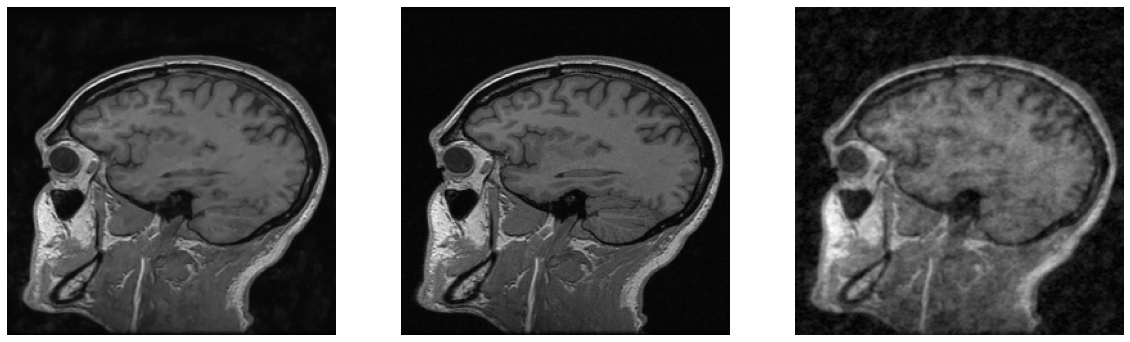
\includegraphics[height=1.5in]{Chapter4/images/res4.png}
    \else
      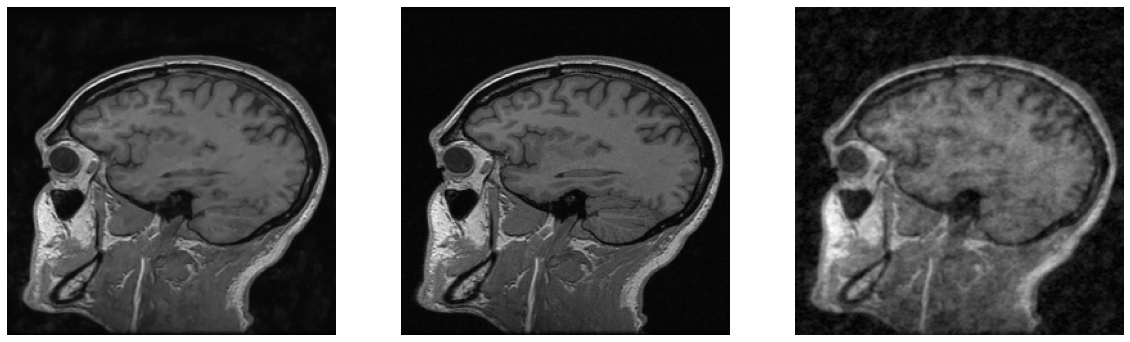
\includegraphics[bb = 92 86 545 742, height=3in]{Chapter4/images/res4.png}
    \fi
    \caption{W-Net 3-layer results -- Predicted (Left), Original (Middle), Undersampled (Right)}
    \label{Result W-Net 3-layer}
  \end{center}
\end{figure}

We trained the model for 25 MRIs and validated it with 10 MRIs. Each MRI has about 170 slices so there are 170-(3-1)=168 inputs (3 slices combine to form one input). Training was done on a Tesla T4 GPU for 30 epochs.\\

As evident from figure \ref{Result W-Net 3-layer} and table \ref{W-Net table}, the model performed on par with the original W-Net and was able to reproduce the fine details such as the folds in the cerebellum, despite the much lesser number of parameters (to fit with the limitations of current hardware) and less number of epochs (75 vs 30). If given better hardware and more time, this model will definitely be able to outperform the original W-Net on the given dataset. This model has a lot of potential and needs to be explored further using better hardware to get exceptional results.


\section{SR3 - Diffusion Model} \label{Observation - SR3}

The SR3 model was trained over a number of different loss functions to improve image super-resolution quality.
\begin{enumerate}
    \item L2 loss
    \item FID
    \item SSIM
    \item FIDR - FID regularized (75\% normalized PSNR, 25\% normalized FID)
    \item SSIMR - SSIM regularized (75\% normalized PSNR, 25\% SSIM)
\end{enumerate}

The following are the results --\\


\begin{table}[h]
\begin{center}
\begin{tabular}{ p{4cm} m{3cm} m{3cm} }
 \hline
 \multicolumn{3}{c}{Comparison table -- SR3} \\
 \hline
 & PSNR & SSIM \\
 \hline
 \hline
 \textbf{Bicubic} & $35.10 \pm 1.22$ & 0.8275\\
 \textbf{L2}    & $34.25 \pm 2.44$ & 0.8233 \\
 \hline
 \textbf{FID}& $35.58 \pm 0.63$  & 0.8354 \\
 \textbf{SSIM}& $36.12 \pm 0.59 $& 0.8618 \\
  \textbf{FIDR}& $36.20 \pm 0.35$  & \textbf{0.8632} \\
 \textbf{SSIMR}& $\bf{36.77 \pm 0.34 }$& 0.8569 \\
 \hline
\end{tabular}
\end{center}
\caption{Comparison between loss functions in SR3}
\label{SR3 table}
\end{table}

FIDR, SSIMR, and Bicubic Interpolation -- all perform at a similar level if seen from the perspective of PSNR (as seen in table \ref{SR3 table}) but PSNR is not able to distinguish well when it comes to scenarios where one image may have distortions or artefacts while another may not and they end up having the same PSNR when compared with the true image.\\

Hence, we will be giving more weightage when it comes to the judgement of quality to SSIM that can capture the perceptual quality of an image in a way that is more similar to humans as compared to PSNR.\\

SSIMR and FIDR models almost perform on a similar level with SSIMR showing the best qualitative results out of all. This shows that having a parameter that gives more weightage to structural similarity performed better as compared to vanilla SR3.\\

The L2 model i.e., the vanilla SR3, and bicubic interpolation showed a decently high PSNR but lagged behind when it came to factors such as structural similarity. Even with the naked eye, one can observe that L2 in Fig. \ref{SR3 L2} wasn't able to give a structurally accurate result when compared to, say, SSIMR in Fig. \ref{Result SR3 - SSIMR}. In the original SR3 paper, they used human subjects and fool rate to get an idea of what image is original when it comes to the judgement of human subjects. Here, we leave the judgement to the reader to observe the difference between the results of these and SSIMR or FIDR.\\

On the other hand, we observed that SSIM and FID seemed to give worse performance than SSIMR of FIDR and also had more noise in their result as compared to the others.\\

Finally, we would like to conclude our observations by saying that the results seem to show that there definitely is a correlation between having a loss function that gives weightage to structural similarity and MRI results that are more structurally similar to the original.

\begin{figure}[!htbp]
  \begin{center}
    \leavevmode
    \ifpdf
      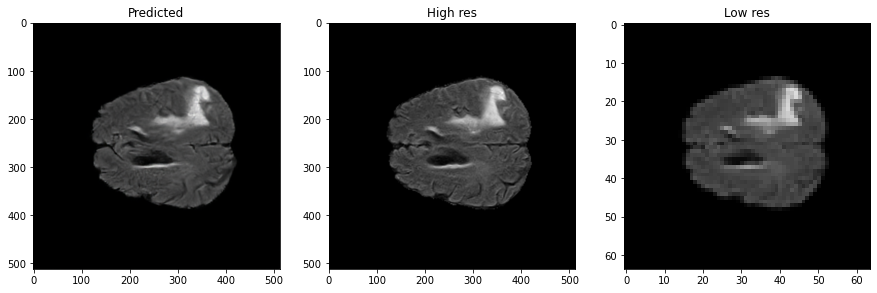
\includegraphics[height=2in]{Chapter4/images/spam1.png}
    \else
      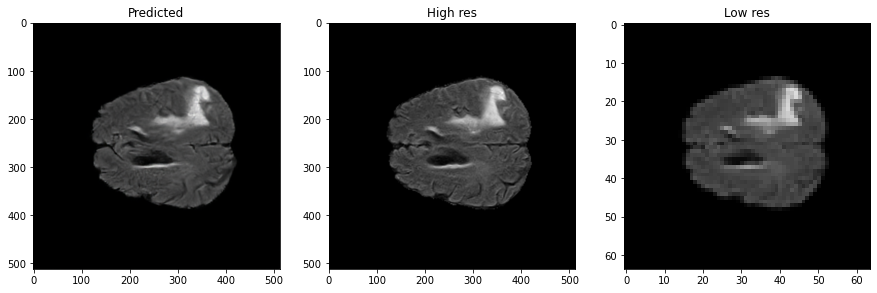
\includegraphics[bb = 92 86 545 742, height=3in]{Chapter4/images/spam1.png}
    \fi
    \caption{SR3 with L2}
    \label{SR3 L2}
  \end{center}
\end{figure} 

\begin{figure}[!htbp]
  \begin{center}
    \leavevmode
    \ifpdf
      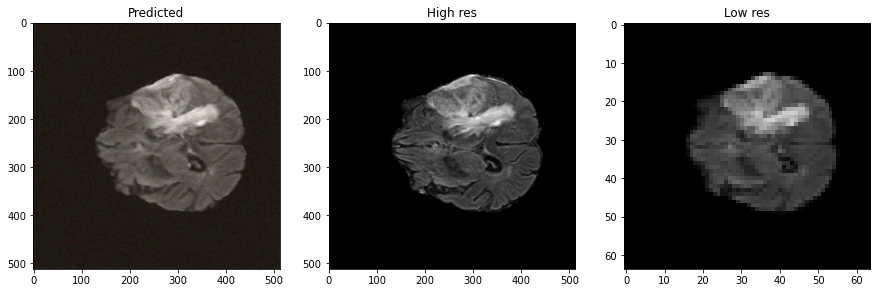
\includegraphics[height=2in]{Chapter4/images/spam3.png}
    \else
      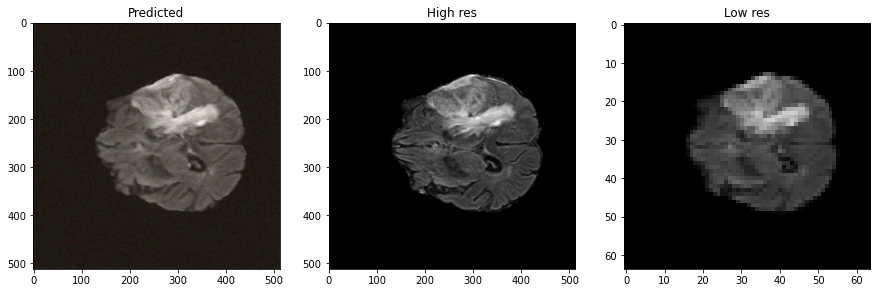
\includegraphics[bb = 92 86 545 742, height=3in]{Chapter4/images/spam3.png}
    \fi
    \caption{SR3 with FID}
    \label{SR3 FID}
  \end{center}
\end{figure} 

\begin{figure}[!htbp]
  \begin{center}
    \leavevmode
    \ifpdf
      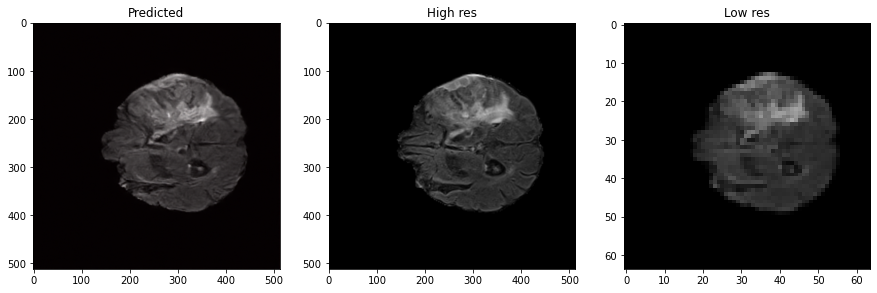
\includegraphics[height=2in]{Chapter4/images/spam2.png}
    \else
      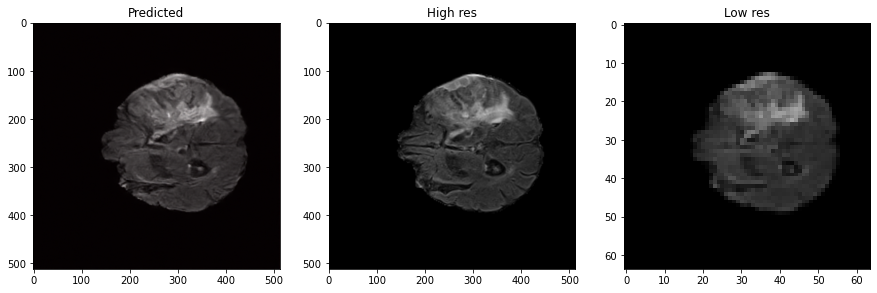
\includegraphics[bb = 92 86 545 742, height=3in]{Chapter4/images/spam2.png}
    \fi
    \caption{SR3 with SSIM}
    \label{SR3 SSIM}
  \end{center}
\end{figure} 



\begin{figure}[!htbp]
  \begin{center}
    \leavevmode
    \ifpdf
      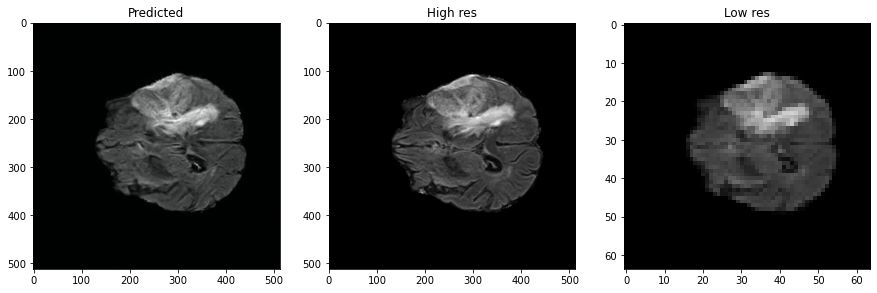
\includegraphics[height=2in]{Chapter4/images/spam4.png}
    \else
      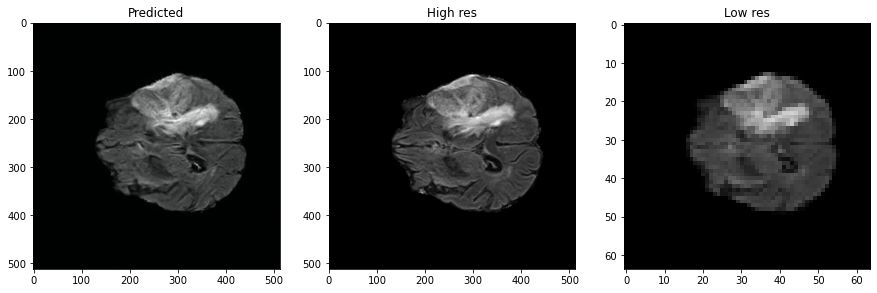
\includegraphics[bb = 92 86 545 742, height=3in]{Chapter4/images/spam4.png}
    \fi
    \caption{SR3 with FIDR}
    \label{SR3 FIDR}
  \end{center}
\end{figure} 


\begin{figure}[!htbp]
  \begin{center}
    \leavevmode
    \ifpdf
      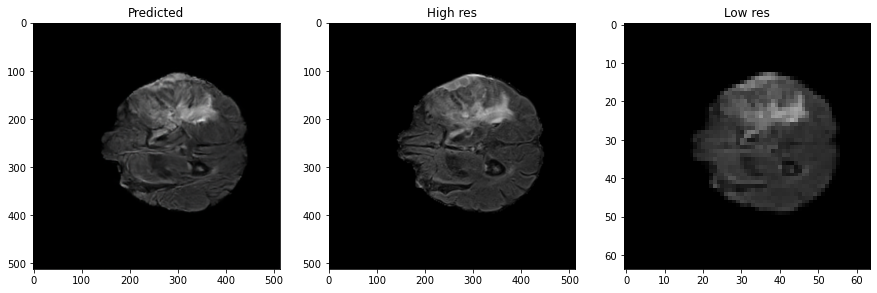
\includegraphics[height=2in]{Chapter4/images/sr3-res1.png}
    \else
      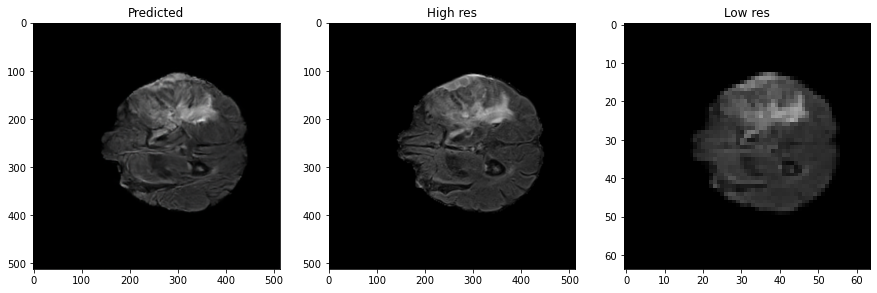
\includegraphics[bb = 92 86 545 742, height=3in]{Chapter4/images/sr3-res1.png}
    \fi
    % \caption{Result 1 }
    % \label{Result 1 W-Net Combined}
  \end{center}

  \begin{center}
    \leavevmode
    \ifpdf
      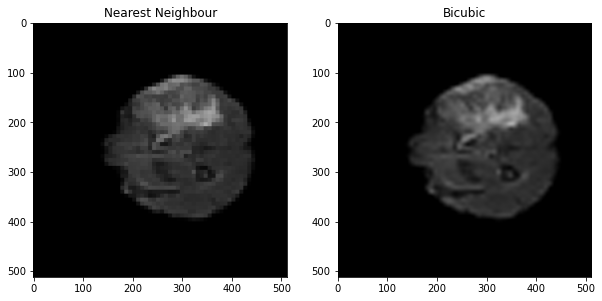
\includegraphics[height=2in]{Chapter4/images/sr3-res2.png}
    \else
      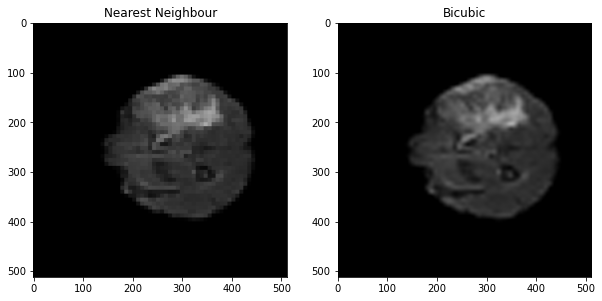
\includegraphics[bb = 92 86 545 742, height=3in]{Chapter4/images/sr3-res2.png}
    \fi
    \caption{SR3 with SSIMR}
    \label{Result SR3 - SSIMR}
  \end{center}
\end{figure}




%%% ----------------------------------------------------------------------

% ------------------------------------------------------------------------

%%% Local Variables: 
%%% mode: latex
%%% TeX-master: "../thesis"
%%% End: 
